%%%%%%%%%%%%%%%%%%%%%%%%%%%%%%%%%%%%%%%%%%%%%%%%%%%%%%%%%%%%%%%%%%%%%%%%%%%%%%%%
%2345678901234567890123456789012345678901234567890123456789012345678901234567890
%        1         2         3         4         5         6         7         8

\documentclass[letterpaper, 10 pt, conference]{ieeeconf}  % Comment this line out if you need a4paper

%\documentclass[a4paper, 10pt, conference]{ieeeconf}  % Use this line for a4 paper

\IEEEoverridecommandlockouts % This command is only needed if  you want to use the \thanks command

\overrideIEEEmargins                                      % Needed to meet printer requirements.

%In case you encounter the following error:
%Error 1010 The PDF file may be corrupt (unable to open PDF file) OR
%Error 1000 An error occurred while parsing a contents stream. Unable to analyze the PDF file.
%This is a known problem with pdfLaTeX conversion filter. The file cannot be opened with acrobat reader
%Please use one of the alternatives below to circumvent this error by uncommenting one or the other
%\pdfobjcompresslevel=0
%\pdfminorversion=4

% See the \addtolength command later in the file to balance the column lengths
% on the last page of the document

\pdfminorversion=5

% Strictly reuse IROS2024-style preamble logic.
\usepackage{epsfig}
\usepackage{graphicx}
\usepackage{amsmath}
\usepackage{amssymb}
\usepackage{color}
\usepackage[linesnumbered,ruled]{algorithm2e}
\usepackage[normalem]{ulem}
\makeatletter
\let\NAT@parse\undefined
\makeatother
\usepackage{hyperref}
\hypersetup{pdfstartview=FitH,
            colorlinks=true,
            linkcolor=red,
            anchorcolor=blue,
            citecolor=green
            }
\usepackage{cite}
\usepackage{booktabs}
\usepackage{multirow}
\usepackage[caption=false,font=footnotesize]{subfig}
\usepackage[dvipsnames,table]{xcolor}
\usepackage{soul}
\usepackage{balance}
\newcounter{RNum}
\renewcommand{\theRNum}{\arabic{RNum}}
\newcommand{\Remark}{\noindent\textit{\textbf{Remark}~\refstepcounter{RNum}\textbf{\theRNum}: }}
\newcommand{\NoOne}[1]{\textcolor{red}{#1}}
\newcommand{\NoTwo}[1]{\textcolor{green}{#1}}
\newcommand{\NoThree}[1]{\textcolor{blue}{#1}}
\soulregister\NoOne7
\soulregister\NoTwo7
\soulregister\NoThree7
\soulregister\Remark7
\definecolor{table_c}{RGB}{245,228,208}

% Keep required packages for this manuscript.
\usepackage{url}
\usepackage{arydshln}
\usepackage{hhline}
\usepackage{pifont}
\usepackage{tikz}
\usepackage{afterpage}
\usepackage{float}
\usepackage{placeins}

% Keep operator style in \mathrm without bold.
% This guarantees operators differ from italic math variables in equations.
\newcommand{\mathopfont}[1]{\mathop{\mathrm{#1}}\nolimits}
% ieeeconf 已定义 \labelindent，与 enumitem 冲突；先解除再加载
\makeatletter
\let\labelindent\relax
\makeatother
\usepackage{enumitem}
\setlist[itemize]{noitemsep, topsep=2pt, parsep=0pt, partopsep=0pt}
\setlength{\dashlinedash}{1.7pt}
\setlength{\dashlinegap}{1.2pt}
\newcommand{\cmark}{\ding{51}} % 定义更漂亮的对勾
\DeclareRobustCommand{\circled}[1]{\tikz[baseline=(char.base)]{\node[shape=circle,draw,inner sep=0.6pt] (char) {\footnotesize #1};}}
\setlength{\floatsep}{5pt plus 1pt minus 2pt}
\setlength{\intextsep}{6pt plus 1pt minus 2pt}
\setlength{\abovedisplayskip}{6pt}
\setlength{\belowdisplayskip}{6pt}
\setlength{\abovedisplayshortskip}{4pt}
\setlength{\belowdisplayshortskip}{4pt}
% Tighten vertical spacing for 8-page limit (IEEE column layout).
\setlength{\parskip}{0pt plus 1pt}
\setlength{\textfloatsep}{6pt plus 1pt minus 2pt}
\setlength{\dbltextfloatsep}{6pt plus 1pt minus 2pt}
\setlength{\dblfloatsep}{4pt plus 1pt minus 2pt}

% Keep table captions in normal sentence case (not small caps/all-caps style).
\makeatletter
\long\def\@makecaption#1#2{%
\ifx\@captype\@IEEEtablestring%
\begin{center}{\footnotesize #1}\\{\footnotesize #2}\end{center}%
\@IEEEtablecaptionsepspace%
\else
\@IEEEfigurecaptionsepspace%
\setbox\@tempboxa\hbox{\footnotesize #1.~~ #2}%
\ifdim \wd\@tempboxa >\hsize%
\setbox\@tempboxa\hbox{\footnotesize #1.~~ }%
\parbox[t]{\hsize}{\footnotesize \noindent\unhbox\@tempboxa#2}%
\else%
\ifcenterfigcaptions \hbox to\hsize{\footnotesize\hfil\box\@tempboxa\hfil}%
\else \hbox to\hsize{\footnotesize\box\@tempboxa\hfil}%
\fi\fi\fi}
\makeatother

\title{\LARGE \bf
MAE-OVD: MAE-Powered Open-Vocabulary Vision-Language Model for Anti-UAV Detection}

\author{Changhong Fu$^{1,*}$, Zhangchi Guo$^{1}$, Liangliang Yao$^{1}$, Haobo Zuo$^{2}$, Mengyuan Li$^{1}$, Yipeng Feng$^{1}$ %  
\thanks{$^{*}$Corresponding author}
\thanks{
$^{1}$C. Fu, Z. Guo, L. Yao, M. Li, and Y. Feng are with the School of Mechanical Engineering, Tongji University, Shanghai 201804, China.
\itshape{Email: changhongfu@tongji.edu.cn}
}
\thanks{
$^{2}$H. Zuo is with the School of Computing and Data Science, The University of Hong Kong, Hong Kong 999077, China.
}
%
}


\begin{document}



\maketitle
\thispagestyle{empty}
\pagestyle{empty}

%%%%%%%%%%%%%%%%%%%%%%%%%%%%%%%%%%%%%%%%%%%%%%%%%%%%%%%%%%%%%%%%%%%%%%%%%%%%%%%
\noindent
\begin{abstract}

Open-vocabulary detection (OVD) is valuable for anti-unmanned aerial vehicle (UAV) applications, as natural-language referring enables rapid, precise instance-level localization. However, existing OVD methods face significant challenges in UAV views due to motion blur, tiny objects, low signal-to-noise ratio, and heavy background clutter, which jointly degrade visual representations and weaken text-visual alignment. To address these challenges, this work proposes a novel OVD framework driven by Masked Autoencoding (MAE) for anti-UAV zero-shot localization. Specifically, an MAE-driven backbone is introduced to reconstruct partially corrupted UAV observations and mine degradation-resistant global structural cues, thereby compensating for missing fine details of tiny or blurred objects and providing more reliable visual semantics for subsequent text-visual alignment. Additionally, by effectively enhancing bidirectional multi-scale text-visual interaction, an innovative path aggregation network and a clear implicit feature semantic distillation module are designed to purify alignment responses and suppress semantic distractors. Moreover, a decoupled train-test pipeline leverages MAE during training while maintaining lightweight deployment. Experimental results on authoritative anti-UAV benchmark demonstrate that MAE-OVD outperforms state-of-the-art detectors. The code is located at \url{https://github.com/vision4robotics/MAE-OVD}.

\end{abstract}

%%%%%%%%%%%%%%%%%%%%%%%%%%%%%%%%%%%%%%%%%%%%%%%%%%%%%%%%%%%%%%%%%%%%%%%%%%%%%%%
\section{Introduction}
\label{sec:introduction}

Open-vocabulary detection (OVD) serves as a crucial task for anti-unmanned aerial vehicle (UAV) systems~\cite{fu_progressive_2024,yao_sgdvit_2023,10015799,9196943}, enabling detectors to localize aerial objects from natural-language descriptions. However, UAV-view scenes~\cite{zhu2019visdrone,lam2018xview,Zuo2022DeconNetED} present significant challenges because motion blur, long-range tiny objects, and heavy background clutter typically occur simultaneously. This challenge is further compounded by the gap between pretraining and deployment environments, where most vision-language models are trained on well-exposed objects, whereas aerial imagery frequently presents only a few informative pixels together with viewpoint distortion and abrupt scale variation. Consequently, even strong open-vocabulary detectors such as OWL-ViT~\cite{minderer2022owlvit} and grounding-based pipelines~\cite{li2022glip,liu2024groundingdino} frequently yield fragile region-text matching when aerial semantics must be recovered from weak visual evidence~\cite{minderer2022owlvit}. \textbf{\textit{Therefore, it is imperative to design an OVD framework that can effectively purify textual information and accurately enhance visual features for anti-UAV.}}

\begin{figure}[!t]
\centering
\includegraphics[width=\columnwidth]{method_compare.pdf}
\vspace{-20pt}
\caption{Qualitative comparison in a real anti-UAV scenario. Fixed-label detectors cannot ground natural-language queries. Existing OVD methods' alignment responses remain spatially diffuse under the challenges. The proposed MAE-OVD sharpens text-visual matching for more accurate zero-shot localization.}
\label{fig:method_compare}
\end{figure}

Most existing anti-UAV methods mainly focus on alleviating degradation-induced text-visual misalignment~\cite{drones9070495,zhu2019visdrone}, and some training strategies further introduce Masked Autoencoding (MAE) reconstruction~\cite{he2022mae,kang2023deblurmae} to improve robustness under degraded imagery, but several critical bottlenecks are still overlooked. In particular, although MAE can recover global structures from corrupted inputs, its pixel-dominant objective is inherently less sensitive to tiny aerial objects that occupy only a few pixels, whose weak semantics are easily submerged by background clutter and diluted by large receptive fields, causing detectors to either miss the object entirely or predict severely biased boxes even when coarse category cues are available. Moreover, rare or long-tail objects remain insufficiently modeled, making the alignment process overly dominated by frequent concepts and increasing confusion with visually similar distractors when uncommon categories appear. This limitation becomes even more evident for rapidly moving UAVs, where abrupt displacement, motion blur, and drastic scale variation further destabilize the already fragile correspondence between sparse visual evidence and language queries. \textbf{\textit{Therefore, anti-UAV methods are required to not only resist image degradation effectively, but also maintain high detection sensitivity towards miniature, low-occurrence and fast-moving objects.}}

Insufficient deep text-visual interaction further limits the quality of zero-shot localization. Efficient path aggregation networks (PAN)~\cite{cheng2024yoloworld,wang2025yoloe} improve efficiency, but the alignment still relies on shallow cross-scale aggregation. In cluttered UAV scenes, this leads to weak semantic consistency across pyramid levels, where descriptions such as "drone" cannot be stably separated from similar distractors including birds, clouds or other aerial objects. In practice, anti-UAV localization requires high-level semantics~\cite{cao_hift_2021} to guide fine-resolution features while preserving spatial selectivity, yet detectors often maintain only category-level confidence and fail to recover precise object extent~\cite{gu2022vild,zhong2022regionclip}. Consequently, robust multi-scale grounding remains difficult. \textbf{\textit{Accordingly, a stronger bidirectional interaction mechanism is necessary to preserve both semantic consistency and localization precision in anti-UAV OVD.}}

Semantic contamination in response maps compromises model reliability by triggering responses not only on the true object but also on irrelevant yet semantically related regions. Although text-visual fusion is available, the alignment map frequently exhibits spatial scatter and over-activation on background regions. Such contamination poses critical hazards in safety-critical anti-UAV systems, as false responses on sky regions, buildings, or moving background objects inevitably interfere with downstream object locking and interception logic. Recent studies on prompt-based semantic priors suggest that distilling implicit text knowledge can improve grounding quality~\cite{implicitknowledge2024,li2025codet}, whereas a stable purification strategy specifically designed for anti-UAV OVD remains absent. \textbf{\textit{Therefore, suppressing semantic distractors in response maps is essential for reliable anti-UAV zero-shot localization.}}

In this work, a novel OVD method is proposed to boost anti-UAV localization under severe degradation and clutter. The main contributions are summarized as follows:
\begin{itemize}
\item A novel OVD for anti-UAV is formulated by coupling degradation-resistant representation learning, deep text-visual interaction, and semantic purification within a decoupled train-test pipeline.
\item Degradation-resistant representation learning is integrated into the training pipeline via a MAE-driven auxiliary-only restoration expert, stabilizing low-level structures under motion blur and low signal-to-noise ratio (SNR) while maintaining detector efficiency.
\item Multi-scale feature bidirectional alignment is organized and enhanced in the PAN and distallition module, enabling the response map purified by task-aware masking and staged optimization for grounding robustness.
\item Extensive experiments on authoritative anti-UAV benchmark demonstrate that the proposed method outperforms existing state-of-the-art (SOTA) methods in both quantitative and qualitative results.
\end{itemize}

\begin{figure*}[!t]
    \centering
    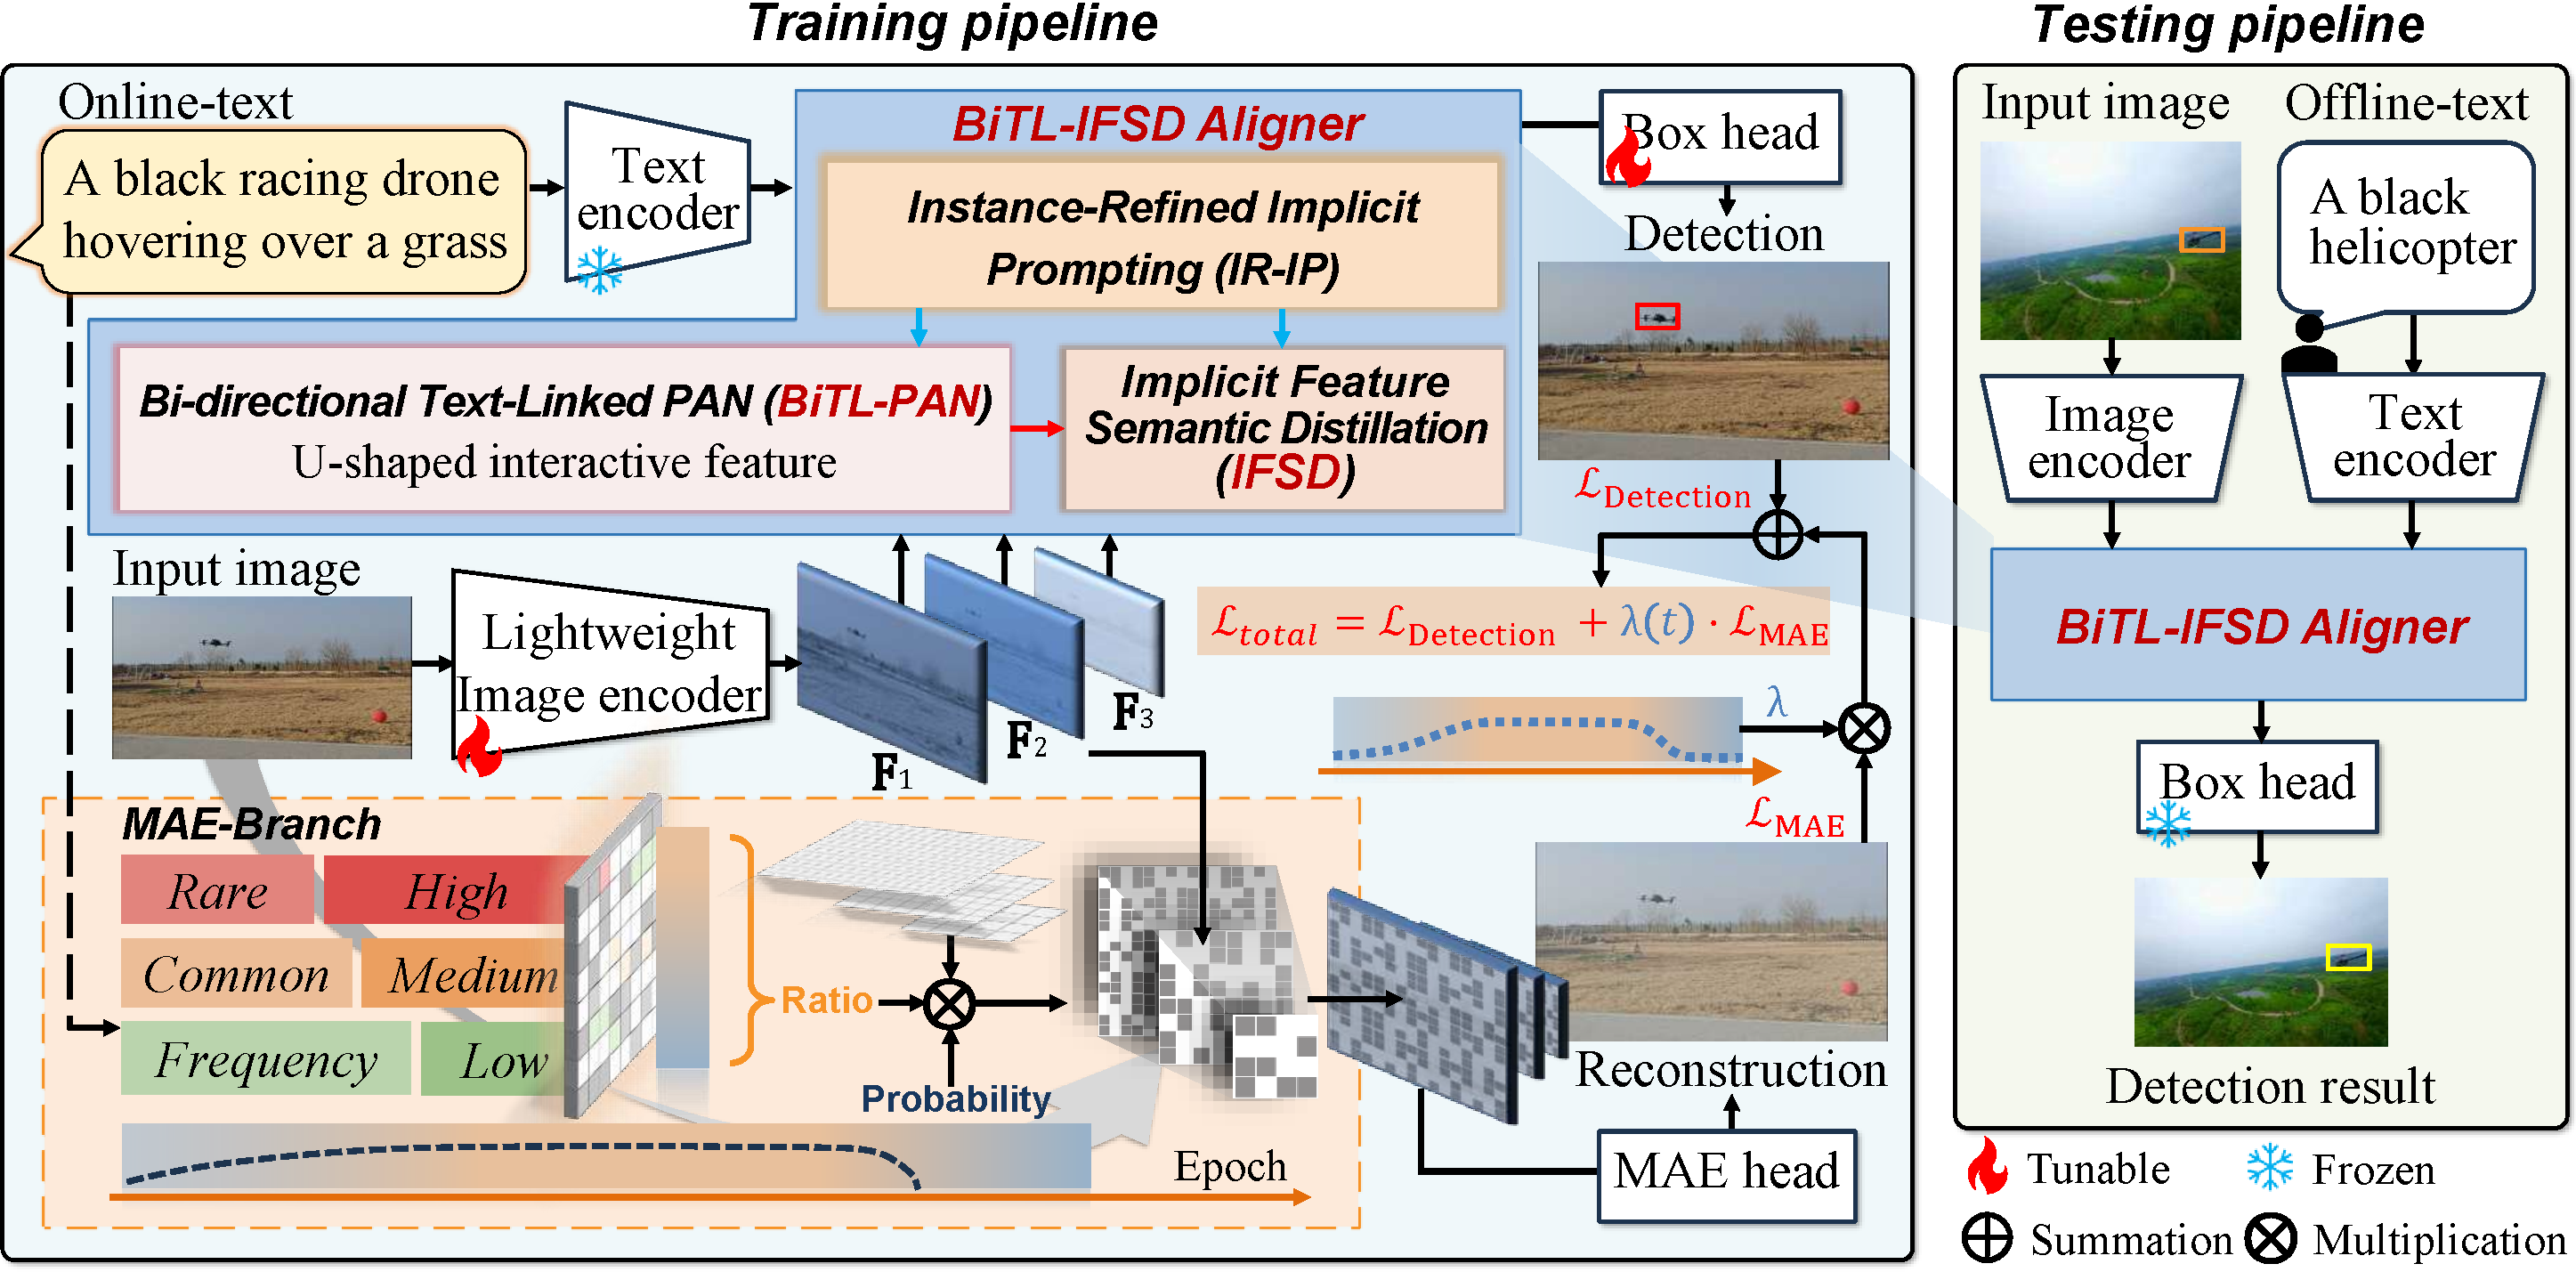
\includegraphics[width=1.0\textwidth]{pipeline.pdf}
    \vspace{-15pt}
    \caption{The overall architecture of the proposed MAE-OVD. \textbf{Left (Train):} Dual-task pipeline with three components. (1) MAE branch: patchify, hierarchical feature masks, lightweight image encoder, MAE reconstruction decoder, and $\mathcal{L}_{\mathrm{MAE}}$. (2) Cross-modal branch: online text, text encoder (frozen), IR-IP, and BiTL-PAN. (3) IFSD and box head with $\mathcal{L}_{\mathrm{Detection}}$. \textbf{Right (Test):} Lightweight inference with offline text, image/text encoders, BiTL-IFSD Aligner, and Box head (frozen) for zero-shot localization.}
    \label{fig:pipeline}
\end{figure*}

\section{Related Work}
\label{sec:related}

\subsection{Anti-UAV and Zero-Shot Localization}
Recent anti-UAV research covers detection, tracking, and multimodal perception under aerial viewpoints, with public benchmarks such as DUT-Anti-UAV, VisDrone, and xView providing diverse scenes and object scales~\cite{zhao2022dutantiuav,zhu2019visdrone,lam2018xview}. Emerging UAV-OVD studies begin to introduce language-conditioned recognition for unseen categories~\cite{cheng2024yoloworld,wang2025mambayoloworld,wang2025yoloe,liu2024groundingdino}. However, most existing anti-UAV pipelines remain built upon closed vocabularies, tracker-dependent assumptions, or dataset-specific tuning, thereby rendering direct text-to-box localization for unseen objects unstable in single-frame settings. Large scale variation, fast motion blur, low SNR, and semantic distractors further amplify this instability, frequently producing scattered activation and class confusion between UAV objects and background objects.

\subsection{Open-Vocabulary Detection}
OVD aligns region-level visual features with text embeddings learned from vision-language pretraining, as exemplified by CLIP~\cite{radford2021clip}, therefore detection is formulated as cross-modal matching rather than fixed-class classification. Representative methods include grounding-oriented transformers such as GLIP~\cite{li2022glip} and Grounding DINO~\cite{liu2024groundingdino}, as well as real-time frameworks such as YOLO-World~\cite{cheng2024yoloworld}, Mamba-YOLO-World~\cite{wang2025mambayoloworld}, and YOLOE~\cite{wang2025yoloe}. The modern OVD stack also inherits key advances from region-based detection and dense supervision, together with transformer detectors and transferable visual backbones~\cite{liu2021swin,carion2020detr}. These methods show strong generalization to unseen categories and enable vocabulary expansion without per-class retraining~\cite{gu2022vild,minderer2022owlvit}, with similar trends reported by DetPro and related prompt-based open-vocabulary studies~\cite{du2022detpro}. However, because most pretraining data come from ground-level internet imagery, the domain gap for count-UAV with tiny instances and heavy clutter often weakens alignment quality and causes large performance drops under blur and distractors~\cite{zhong2022regionclip}.

\subsection{MAE and Training Strategy}
MAE reconstructs masked patches from partial observations and forces encoders to model global structure~\cite{he2022mae}. This mechanism has been extended to deblurring-oriented pretraining~\cite{kang2023deblurmae}. However, existing MAE studies mainly optimize restoration quality or generic representation learning, and evaluations are usually conducted in closed-set classification or reconstruction protocols. Under open-vocabulary UAV detection, the coupling between restoration-oriented pretext learning and text-conditioned localization remains underexplored, and robustness gains from MAE are not consistently transferred to cross-modal matching quality.

\section{MAE-OVD: Architecture and Pipeline}
\label{sec:method}

\afterpage{%
\begin{figure*}[!t]
    \centering
    \includegraphics[width=1.0\textwidth]{sub_pipeline.pdf}
    \vspace{-18pt}
    \caption{Bi-directional Text-Linked PAN and Implicit Feature Semantic Distillation sub-pipeline.}
    \label{fig:sub_pipeline}
\end{figure*}
}

The decoupled train-test pipeline of MAE-OVD is designed for anti-UAV as illustrated in Fig.~\ref{fig:pipeline} under motion blur, tiny objects, low-SNR observations, and heavy background clutter, without extra inference overhead.

For notation, given an input image $\mathbf{I} \in \mathbb{R}^{3 \times H \times W}$, $H$ and $W$ denote height and width. Multi-scale features $\mathbf{F}_1,\mathbf{F}_2,\mathbf{F}_3$ (shallow to deep) are produced by the lightweight encoder, with $\mathbf{F}_i\in\mathbb{R}^{B\times C_i\times H_i\times W_i}$, batch size $B$, and $C_i$, $H_i$, $W_i$ the channel count, height, and width at scale $i$. The frozen text embedding is $\mathbf{y}\in\mathbb{R}^{B\times d}$, where $d$ is the text embedding dimension. Refined, instance-conditioned, and text-enhanced forms are denoted $\mathbf{Y}\in\mathbb{R}^{B\times d}$, $\mathbf{F}'_3$, and $\mathbf{F}_{iY}$.

\subsection{Overall Pipeline}

MAE-OVD consists of three components: an MAE-driven branch for degradation-resistant representation learning, a bi-directional text-linked PAN (BiTL-PAN) for multi-scale text-visual interaction, and an implicit
feature semantic distallition (IFSD) module for semantic purification. During training, the image is encoded into $\mathbf{F}_1,\mathbf{F}_2,\mathbf{F}_3$, text embeddings are refined by Instance-reffned implicit prompting (IR-IP), and the resulting cross-modal features are aggregated by BiTL-PAN, purified by IFSD, and fed to the box head. In parallel, the MAE branch reconstructs masked observations to regularize the shared encoder.

During inference, the MAE decoder and all reconstruction-only components are discarded. Given an image and precomputed text embeddings, the trained image encoder, the BiTL-IFSD Aligner, and the box head perform one-pass localization. In this way, the robustness induced by restoration-oriented supervision is preserved without repeated image reconstruction or prompt processing, which is well suited for efficient onboard anti-UAV deployment.

\noindent\textbf{\textit{Remark 1:}} The decoupled train-test is designed to treat the UAV-view noise and scale issues as the primary focus of training. By concentrating restoration-oriented supervision on these deployment-critical degradations, MAE-OVD learns representations that transfer efficiently to inference, while still preserving a lightweight one-pass detector without extra reconstruction overhead.

\subsection{Training Strategy}
\label{subsec:mae-backbone}

The training strategy is centered on an MAE-driven backbone acting as a restoration expert~\cite{he2022mae,kang2023deblurmae}. Because UAV objects are often tiny, blurred, and cluttered, box supervision alone is insufficient to recover reliable evidence. The auxiliary MAE objective encourages the shared encoder to infer missing structures from incomplete observations, yielding degradation-resistant contour, shape, and layout cues that transfer to text-conditioned localization.

Given image $\mathbf{I} \in \mathbb{R}^{3 \times H \times W}$, non-overlapping $P \times P$ patches are generated and a binary mask $\mathcal{M}$ with ratio $\rho$ is sampled. The same mask is propagated across all pyramid levels. At scale $s$, the propagated mask $\mathbf{M}^{(s)} \in \{0,1\}^{H_s \times W_s}$ is broadcast along channels, where $\mathbf{M}^{(s)}_{ij}=1$ and $\mathbf{M}^{(s)}_{ij}=0$ denote masked and visible locations, respectively. The mask-aware feature is defined as:
\begin{equation}
\mathbf{\tilde{F}}_{\mathrm{s}} = \mathbf{F}_s \odot (1 - \mathbf{M}^{(s)}) + \mathbf{E}^{(s)}_{\mathrm{mask}} \odot \mathbf{M}^{(s)} \quad,
\end{equation}
where $\mathbf{\tilde{F}}_{\mathrm{s}}$ is the mask-aware feature, $\mathbf{F}_s$ is the original feature map, and $\mathbf{E}^{(s)}_{\mathrm{mask}}$ is a learnable mask token with the same shape as $\mathbf{F}_s$. Visible observations are preserved and missing regions are replaced with trainable placeholders, therefore weak structures are recovered from context at each level. A shared mask across the pyramid yields consistent visibility priors between shallow and deep features and aligns tiny-object detail with high-level semantics.


Beyond random masking, a frequency-aware policy is adopted to emphasize underrepresented structures. The random masking ratio is set to $0.4$ during joint detector training with Mosaic augmentation and $0.5$ during MAE-focused pretraining with Mosaic. For long-tailed open-vocabulary data, semantic masking further uses ratios of $0.4$, $0.1$, and $0.0$ for rare, common, and frequent categories, respectively, and $0.6$ for background regions. This design allocates more reconstruction capacity to weak or uncommon objects while discouraging reliance on cluttered backgrounds.

The reconstruction branch feeds fused $\mathbf{F}_1/\mathbf{F}_2/\mathbf{F}_3$ features into the decoder, so that masked restoration can exploit both fine spatial detail and high-level semantics. Supervision is applied only on masked patches:
\begin{equation}
\mathcal{L}_{\mathrm{MAE}} = \frac{1}{|\mathcal{M}|} \sum_{p \in \mathcal{M}} \| \hat{\mathbf{I}}_p - \mathbf{I}_p \|_2^2 \quad,
\end{equation}
where $\mathcal{M}$ is the set of masked patch indices, $|\mathcal{M}|$ is the number of masked patches, $\hat{\mathbf{I}}_p$ is the reconstructed RGB vector of patch $p$, and $\mathbf{I}_p$ is the ground-truth RGB vector. The overall optimization objective is:
\begin{equation}
\mathcal{L}_{\mathrm{total}} = \mathcal{L}_{\mathrm{Detection}} + \lambda(t)\,\mathcal{L}_{\mathrm{MAE}} \quad,
\end{equation}
where $\mathcal{L}_{\mathrm{Detection}}$ is the detection loss and $\lambda(t)$ is a time-dependent balance factor. In the main setting, $\lambda(0)=0.1$ and can be increased to $0.2$ during the early stage of training. The MAE branch is activated with probability $p_{\mathrm{mae}}=0.35$ per batch and progressively weakened after a one-epoch warmup: $\lambda(t)$ decays to zero, Mosaic is disabled in the final stage, and the MAE branch is removed in the last two epochs. Therefore, early training emphasizes degradation-resistant structure recovery, whereas late training focuses on box regression and text-visual matching. The text encoder remains frozen, while the image encoder, IR-IP, BiTL-PAN, IFSD, and Box head are optimized end-to-end.

\noindent\textbf{\textit{Remark 2:}} By introducing MAE supervision before text-visual alignment and using different masking strengths for objects and backgrounds, the model emphasizes small objects and reduces clutter dependency, improving robustness to background interference and long-tail bias.

\subsection{BiTL-IFSD}

\subsubsection{BiTL-PAN: The U-shaped Interaction Hub}
\label{subsec:bitl-pan}
IR-IP refines text embedding $\mathbf{y}$ with the visual context of deep feature $\mathbf{F}_3$. Let $\bar{\mathbf{v}}=\mathopfont{GAP}(\mathbf{F}_3)$, then following the MHA block in Fig.~\ref{fig:sub_pipeline}, utilize $\mathbf{y}$ as the query and $\bar{\mathbf{v}}$ as both key and value. To enable cross-modal interaction, $\bar{\mathbf{v}}$ is projected to match the text embedding dimension. Rather than treating the prompt as a fixed class descriptor, this module performs image-conditioned residual refinement:
\begin{align}
\bar{\mathbf{v}}' &= \mathopfont{Linear}(\bar{\mathbf{v}}) \quad, \\
\mathbf{Y} &= \mathopfont{LayerNorm}\!\left( \mathopfont{Att}(\mathbf{y},\bar{\mathbf{v}}',\bar{\mathbf{v}}') \right) \oplus \mathbf{y} \quad, \\
\mathbf{F}'_3 &= \mathopfont{Broadcast}\!\left( \bar{\mathbf{v}} \otimes \mathopfont{Linear}(\mathbf{y}) \right) \quad,
\end{align}
where $\bar{\mathbf{v}}$ denotes the global pooled visual descriptor from $\mathbf{F}_3$, $\bar{\mathbf{v}}'$ denotes the projected visual descriptor, $\mathopfont{GAP}(\cdot)$ denotes global average pooling, $\mathopfont{Att}(\mathbf{Q},\mathbf{K},\mathbf{V})=\mathopfont{Softmax}\big( \frac{\mathbf{Q}\mathbf{K}^\top}{\sqrt{\mathrm{d}}} \big)\mathbf{V}$ denotes the scaled dot-product attention shown in Fig.~\ref{fig:sub_pipeline}, $\mathopfont{LayerNorm}(\cdot)$ denotes layer normalization, $\oplus$ denotes element-wise addition, $\otimes$ denotes element-wise multiplication, $\mathopfont{Broadcast}(\cdot)$ expands the channel vector to spatial dimensions, $\mathrm{d}$ denotes the text embedding dimension, and $\mathbf{Y}$ denotes the refined text embedding, and $\mathopfont{Linear}: \mathbb{R}^{d} \rightarrow \mathbb{R}^{C_3}$ projects the text embedding to match $\bar{\mathbf{v}}$ for element-wise fusion. Afterwards, $\bar{\mathbf{v}} \otimes \mathopfont{Linear}(\mathbf{y})$ fuses the globally pooled visual context with a linear-projected text embedding, thereby preserving original text semantics while introducing image-conditioned correction. This effect is important under partial blur or sub-pixel extent, where rigid prototypes are easily attracted to semantically similar background regions.

BiTL-PAN performs bidirectional interaction over $\mathbf{F}_1,\mathbf{F}_2,\mathbf{F}_3$ with refined text embedding $\mathbf{Y}$ from IR-IP, following a U-shaped interactive flow:

Top-down (semantic injection): $\mathbf{F}_3$ and $\mathbf{F}'_3$ interact as $(\mathbf{F}_i,\mathbf{F}_j)$, the intermediate product is upsampled for interaction with $\mathbf{F}_2$. Then the second intermediate product is upsampled for interaction with $\mathbf{F}_1$ to produce $\mathbf{F}_{1Y}$.

Bottom-up (localization recovery): $\mathbf{F}_{1Y}$ is downsampled for interaction with the second product from top-down flow to obtain $\mathbf{F}_{2Y}$, which is afterwards downsampled for interaction with the first product to produce $\mathbf{F}_{3Y}$.

For each scale, the current feature $\mathbf{F}_i$ and adjacent-scale feature $\mathbf{F}_j$ are concatenated and modulated by a text-guided spatial gate $\mathbf{M}_{ij}$:
\begin{align}
\tilde{\mathbf{C}}_{ij} &= [\mathbf{F}_i; \mathbf{F}_j] \quad, \\
\boldsymbol{\gamma} &=\mathopfont{Linear}(\mathbf{Y}) \quad, \\
\mathbf{M}_{ij} &= \sigma\big( \boldsymbol{\gamma} \otimes \mathopfont{Conv}_{1\times1}(\tilde{\mathbf{C}}_{ij}) \big) \quad, \\
\mathbf{F}_{iY} &= \tilde{\mathbf{C}}_{ij} \otimes \mathbf{M}_{ij} \oplus \mathopfont{Conv}_{1\times1}(\tilde{\mathbf{C}}_{ij}) \quad,
\end{align}
where $[\cdot ; \cdot]$ denotes channel-wise concatenation, $\mathopfont{Conv}_{1\times1}$ is a $1\times1$ convolution, $\sigma(\cdot)$ denotes the sigmoid function, $\tilde{\mathbf{C}}_{ij}$ represents the concatenated adjacent-scale feature, $\boldsymbol{\gamma}$ denotes the text-guided gate scalar broadcast to spatial dimensions, $\mathbf{M}_{ij}$ denotes the spatial mask generated by channel-text fusion, and $\mathbf{F}_{iY}$ represents the text-enhanced feature at level $i$, consistent with Fig.~\ref{fig:sub_pipeline}. The spatial mask emphasizes object-relevant regions while suppressing clutter-induced activations. The residual path ensures that faint UAV evidence is not over-suppressed, maintaining detection sensitivity under incomplete or blurred appearance.

\subsubsection{IFSD: Semantic Purification Hub}
\label{subsec:ifsd}

IFSD serves as the semantic purification hub~\cite{implicitknowledge2024,li2025codet}. BiTL-PAN interaction features and refined implicit prompts from IR-IP are fused, and semantic distillation is performed to improve localization under complex backgrounds. Semantically related distractors (\textit{e.g.}, birds, clouds, buildings) are common in anti-UAV scenes. Purification is required to concentrate the response on the true object. After multi-scale interaction, visually plausible yet semantically ambiguous responses are explicitly suppressed by IFSD before localization by the box head.

As shown by \circled{C} in Fig.~\ref{fig:sub_pipeline}, $\mathbf{F}_{1Y}$, $\mathbf{F}_{2Y}$, and $\mathbf{F}_{3Y}$ contain different channel counts and spatial resolutions. Each $\mathbf{F}_{iY}$ is first projected to a unified channel dimension $C$ via $\mathopfont{Conv}_{1\times1}^{(i)}:\mathbb{R}^{C_i}\rightarrow\mathbb{R}^{C}$ and then upsampled to the target resolution $H\times W$ via bilinear interpolation. The concatenated result is $\mathbf{R}^{c}=[\mathbf{F}_{1Y};\mathbf{F}_{2Y};\mathbf{F}_{3Y}]$, which is further projected to $\mathbf{F}_{\mathrm{fused}}$ via $\mathopfont{Conv}_{1\times1}$. The refined text embedding $\mathbf{Y}$ is projected to $\mathbf{Y}_{\mathrm{proj}}$. The alignment response is:
\begin{align}
\mathbf{M}_{\mathrm{raw}} &= \mathbf{F}_{\mathrm{fused}} \cdot \mathbf{Y}_{\mathrm{proj}}^\top \quad, \\
\mathbf{M}_A &= \sigma(\mathbf{M}_{\mathrm{raw}}) \quad,
\end{align}
where $\cdot$ denotes the channel-wise inner product between the local feature vector at each spatial location and $\mathbf{Y}_{\mathrm{proj}}$, $\mathbf{M}_{\mathrm{raw}}$ denotes the unnormalized alignment score map, and $\mathbf{M}_A$ represents the normalized response map after sigmoid activation. False positives remain abundant when weak object evidence overlaps cloud edges, bird silhouettes, or building contours. $\mathbf{M}_A$ is sharpened by IFSD through retention of responses jointly supported by visual structure and prompt semantics, improving semantic confidence and spatial reliability. For tiny or partially blurred UAVs, weak sparse peaks are preserved against large-area background activation.
\subsubsection{BiTL-IFSD Aligner}

In the testing stage, the BiTL-IFSD Aligner constitutes the central component of the inference framework. Image features and offline text embeddings are supplied as input, and learned text-visual interaction and semantic purification priors are reused without reintroducing the MAE branch. Unlike heavier grounding frameworks that process text-image pairs online at each step, the proposed aligner follows a real-time OVD deployment schedule while retaining training-time robustness. Aligned features are passed to the box head for one-pass zero-shot localization on onboard or edge anti-UAV platforms under latency and power constraints. Sensitivity to tiny, blurred, low-contrast objects is maintained without the cost of online reconstruction or redundant prompt processing.

\noindent\textbf{\textit{Remark 3:}} By inserting a dedicated purification after multi-scale interaction, BiTL-IFSD prevents semantically related background regions from contaminating the final grounding response, which is essential in cluttered aerial scenes.

\section{Experiments}
\label{sec:experiments}

\subsection{Datasets and Evaluation Protocol}
\label{subsec:datasets-protocol}

Experiments are conducted on the UAV-Anti-UAV benchmark~\cite{zhang2025uavantiuav}. The original release is a million-scale tracking benchmark organized as per-sequence folders with videos and sequence-level annotations. To support open-vocabulary object detection, the dataset is converted into a single-frame detection benchmark by extracting the first valid frame from each sequence with corresponding object box, then reclassify the retained samples into five categories: Fixed\_wing, FPV, Multi\_rotor, VTOL, and Helicopter. The released split contains 1400 training sequences and 420 test sequences.

For detection, the resulting tracking-to-detection conversion is formatted as a COCO-style 5-class benchmark. Sequences with absent first-frame targets are excluded, and samples outside the above five categories are discarded, yielding 419 labeled test images. Metrics follow the COCO protocol, including AP, AP$_{50}$, and AP$_{75}$; for scale-aware analysis, we further report AP$_l$, AP$_m$, AP$_s$, and AvgAP.

\subsection{Implementation Details}

YOLO-World v2 with YOLOv8-S/L and a frozen CLIP ViT-B/32 text encoder processes $640\times640$ inputs: detection uses unmasked images, whereas the MAE branch applies $16\times16$ masking to form $40\times40$ tokens. The MAE decoder takes fused $\mathbf{F}_1/\mathbf{F}_2/\mathbf{F}_3$ features, which are projected to a unified 256-dimensional embedding before reconstruction.

Experiments are run on an Intel Xeon Silver 4214 CPU, and four NVIDIA A100-PCIE-40GB GPUs. Optimization uses AdamW with learning rate $4\times10^{-4}$ and weight decay $0.05$, with optional large-scale detection pretraining (\textit{e.g.}, Objects365~\cite{shao2019objects365}). In the inference stage, the retained components include the image encoder, text encoder, BiTL-IFSD aligner, and box head. Precomputed text embeddings constrain the online inference pathway to exclusively employ the visual backbone and alignment procedure.

\clearpage
\begin{table*}[!p]
\centering
\caption{Detection results on five UAV categories. Metrics: AP, AP$_{50}$, AP$_{75}$, AP$_l$/AP$_m$/AP$_s$, AvgAP. OV/FL and top-three AvgAP per category in red/green/blue follow Sec.~\ref{subsec:quantitative-protocol}. ``--'': omitted entries.}
\vspace{-8pt}
\label{tab:uav-anti-results}
\scriptsize
\renewcommand{\arraystretch}{1.2}
\setlength{\tabcolsep}{9.2pt}
\begin{tabular}{l|lll|cccccc|c}
\hline
\multirow{2}{*}{Category} & \multicolumn{3}{c|}{Method Setting} & \multicolumn{6}{c|}{AP Metrics} & \multirow{2}{*}{AvgAP} \\
\cline{2-10}
 & Method & Backbone & Type & AP & AP$_{50}$ & AP$_{75}$ & AP$_l$ & AP$_m$ & AP$_s$ &  \\
\hline
\multirow{13}{*}{Fixed\_wing} & YOLOv8s & YOLOv8-S & FL & 0.148 & 0.264 & 0.141 & 0.231 & 0.330 & 0.085 & 0.215 \\
 & YOLOv8l & YOLOv8-L & FL & 0.207 & 0.355 & 0.198 & 0.347 & 0.412 & 0.116 & 0.292 \\
\cline{2-11}
 & Grounding DINO~\cite{liu2024groundingdino} & SWIN-T & OV & 0.094 & 0.148 & 0.098 & 0.467 & 0.298 & 0.074 & 0.280 \\
 & MDETR~\cite{kamath2021mdetr} & RN101 & OV & 0.028 & 0.053 & 0.021 & 0.265 & 0.092 & 0.006 & 0.121 \\
 & GLIP~\cite{li2022glip} & SWIN-T & OV & 0.135 & 0.204 & 0.150 & 0.393 & 0.370 & 0.118 & \textbf{\textcolor{blue}{0.294}} \\
 & YOLO-World-S~\cite{cheng2024yoloworld} & YOLOv8-S & OV & 0.076 & 0.126 & 0.068 & 0.351 & 0.176 & 0.036 & 0.188 \\
 & YOLO-World-L~\cite{cheng2024yoloworld} & YOLOv8-L & OV & 0.140 & 0.208 & 0.156 & 0.300 & 0.320 & 0.084 & 0.235 \\
 & Mamba-YOLO-World-S~\cite{wang2025mambayoloworld} & YOLOv8-S & OV & 0.061 & 0.098 & 0.071 & 0.276 & 0.139 & 0.039 & 0.151 \\
 & Mamba-YOLO-World-L~\cite{wang2025mambayoloworld} & YOLOv8-L & OV & 0.027 & 0.077 & 0.013 & 0.038 & 0.106 & 0.019 & 0.054 \\
 & YOLOE-S~\cite{wang2025yoloe} & YOLOv8-S & OV & 0.017 & 0.019 & 0.018 & 0.175 & 0.038 & 0.000 & 0.071 \\
 & YOLOE-L~\cite{wang2025yoloe} & YOLOv8-L & OV & 0.007 & 0.009 & 0.007 & 0.031 & 0.041 & 0.000 & 0.024 \\
\hhline{~----------}
\rowcolor{gray!15}\cellcolor{white} & \textbf{MAE-OVD-S (Ours)} & YOLOv8-S & OV & 0.153 & 0.306 & 0.143 & 0.542 & 0.332 & 0.066 & \textbf{\textcolor{green}{0.313}} \\
\rowcolor{gray!15}\cellcolor{white} & \textbf{MAE-OVD-L (Ours)} & YOLOv8-L & OV & \textbf{0.210} & \textbf{0.413} & 0.187 & \textbf{0.590} & \textbf{0.416} & \textbf{0.123} & \textbf{\textcolor{red}{0.376}} \\
\hline\hline
\multirow{13}{*}{FPV} & YOLOv8s & YOLOv8-S & FL & 0.040 & 0.090 & 0.013 & -- & 0.003 & 0.050 & 0.027 \\
 & YOLOv8l & YOLOv8-L & FL & 0.047 & 0.097 & 0.038 & -- & 0.000 & 0.040 & 0.020 \\
\cline{2-11}
 & Grounding DINO~\cite{liu2024groundingdino} & SWIN-T & OV & 0.035 & 0.060 & 0.044 & -- & 0.195 & 0.059 & 0.127 \\
 & MDETR~\cite{kamath2021mdetr} & RN101 & OV & 0.004 & 0.020 & 0.000 & -- & 0.028 & 0.009 & 0.019 \\
 & GLIP~\cite{li2022glip} & SWIN-T & OV & 0.013 & 0.024 & 0.009 & -- & 0.155 & 0.057 & 0.106 \\
 & YOLO-World-S~\cite{cheng2024yoloworld} & YOLOv8-S & OV & 0.012 & 0.039 & 0.008 & -- & 0.042 & 0.015 & 0.029 \\
 & YOLO-World-L~\cite{cheng2024yoloworld} & YOLOv8-L & OV & 0.060 & 0.119 & 0.054 & -- & 0.135 & 0.049 & 0.092 \\
 & Mamba-YOLO-World-S~\cite{wang2025mambayoloworld} & YOLOv8-S & OV & 0.077 & 0.132 & 0.066 & -- & 0.219 & 0.052 & \textbf{\textcolor{green}{0.136}} \\
 & Mamba-YOLO-World-L~\cite{wang2025mambayoloworld} & YOLOv8-L & OV & 0.048 & 0.184 & 0.026 & -- & 0.247 & 0.018 & \textbf{\textcolor{blue}{0.133}} \\
 & YOLOE-S~\cite{wang2025yoloe} & YOLOv8-S & OV & 0.004 & 0.005 & 0.006 & -- & 0.137 & 0.000 & 0.069 \\
 & YOLOE-L~\cite{wang2025yoloe} & YOLOv8-L & OV & 0.000 & 0.000 & 0.000 & -- & 0.000 & 0.000 & 0.000 \\
\hhline{~----------}
\rowcolor{gray!15}\cellcolor{white} & \textbf{MAE-OVD-S (Ours)} & YOLOv8-S & OV & 0.050 & 0.116 & 0.019 & -- & 0.099 & 0.054 & 0.077 \\
\rowcolor{gray!15}\cellcolor{white} & \textbf{MAE-OVD-L (Ours)} & YOLOv8-L & OV & \textbf{0.133} & \textbf{0.214} & \textbf{0.169} & -- & \textbf{0.534} & \textbf{0.060} & \textbf{\textcolor{red}{0.297}} \\
\hline\hline
\multirow{13}{*}{Multi\_rotor} & YOLOv8s & YOLOv8-S & FL & 0.070 & 0.120 & 0.072 & 0.298 & 0.250 & 0.020 & 0.189 \\
 & YOLOv8l & YOLOv8-L & FL & 0.099 & 0.178 & 0.096 & 0.354 & 0.282 & 0.050 & \textbf{\textcolor{blue}{0.229}} \\
\cline{2-11}
 & Grounding DINO~\cite{liu2024groundingdino} & SWIN-T & OV & 0.134 & 0.207 & 0.151 & 0.187 & 0.553 & 0.113 & \textbf{\textcolor{green}{0.284}} \\
 & MDETR~\cite{kamath2021mdetr} & RN101 & OV & 0.020 & 0.050 & 0.007 & 0.016 & 0.164 & 0.024 & 0.068 \\
 & GLIP~\cite{li2022glip} & SWIN-T & OV & 0.080 & 0.119 & 0.093 & 0.048 & 0.447 & 0.090 & 0.195 \\
 & YOLO-World-S~\cite{cheng2024yoloworld} & YOLOv8-S & OV & 0.041 & 0.097 & 0.024 & 0.053 & 0.163 & 0.038 & 0.085 \\
 & YOLO-World-L~\cite{cheng2024yoloworld} & YOLOv8-L & OV & 0.035 & 0.090 & 0.025 & 0.141 & 0.108 & 0.021 & 0.090 \\
 & Mamba-YOLO-World-S~\cite{wang2025mambayoloworld} & YOLOv8-S & OV & 0.052 & 0.096 & 0.042 & 0.051 & 0.152 & 0.060 & 0.088 \\
 & Mamba-YOLO-World-L~\cite{wang2025mambayoloworld} & YOLOv8-L & OV & 0.054 & 0.155 & 0.031 & 0.019 & 0.203 & 0.046 & 0.089 \\
 & YOLOE-S~\cite{wang2025yoloe} & YOLOv8-S & OV & 0.013 & 0.027 & 0.007 & 0.017 & 0.145 & 0.021 & 0.061 \\
 & YOLOE-L~\cite{wang2025yoloe} & YOLOv8-L & OV & 0.023 & 0.062 & 0.016 & 0.051 & 0.151 & 0.000 & 0.067 \\
\hhline{~----------}
\rowcolor{gray!15}\cellcolor{white} & \textbf{MAE-OVD-S (Ours)} & YOLOv8-S & OV & 0.065 & 0.120 & 0.065 & 0.072 & 0.227 & 0.067 & 0.122 \\
\rowcolor{gray!15}\cellcolor{white} & \textbf{MAE-OVD-L (Ours)} & YOLOv8-L & OV & \textbf{0.173} & \textbf{0.343} & \textbf{0.154} & \textbf{0.436} & \textbf{0.583} & \textbf{0.132} & \textbf{\textcolor{red}{0.384}} \\
\hline\hline
\multirow{13}{*}{VTOL} & YOLOv8s & YOLOv8-S & FL & -- & -- & -- & -- & -- & -- & -- \\
 & YOLOv8l & YOLOv8-L & FL & -- & -- & -- & -- & -- & -- & -- \\
\cline{2-11}
 & Grounding DINO~\cite{liu2024groundingdino} & SWIN-T & OV & 0.693 & 0.912 & 0.745 & 0.899 & 0.631 & 0.295 & \textbf{\textcolor{green}{0.608}} \\
 & MDETR~\cite{kamath2021mdetr} & RN101 & OV & 0.109 & 0.158 & 0.121 & 0.196 & 0.134 & 0.009 & 0.113 \\
 & GLIP~\cite{li2022glip} & SWIN-T & OV & 0.452 & 0.547 & 0.524 & 0.808 & 0.370 & 0.030 & 0.403 \\
 & YOLO-World-S~\cite{cheng2024yoloworld} & YOLOv8-S & OV & 0.485 & 0.654 & 0.482 & 0.731 & 0.397 & 0.000 & 0.376 \\
 & YOLO-World-L~\cite{cheng2024yoloworld} & YOLOv8-L & OV & 0.572 & 0.803 & 0.604 & 0.860 & 0.443 & 0.126 & 0.476 \\
 & Mamba-YOLO-World-S~\cite{wang2025mambayoloworld} & YOLOv8-S & OV & 0.577 & 0.736 & 0.670 & 0.855 & 0.485 & 0.000 & 0.447 \\
 & Mamba-YOLO-World-L~\cite{wang2025mambayoloworld} & YOLOv8-L & OV & 0.533 & 0.901 & 0.479 & 0.831 & 0.358 & 0.276 & \textbf{\textcolor{blue}{0.488}} \\
 & YOLOE-S~\cite{wang2025yoloe} & YOLOv8-S & OV & 0.399 & 0.452 & 0.452 & 0.692 & 0.295 & 0.000 & 0.329 \\
 & YOLOE-L~\cite{wang2025yoloe} & YOLOv8-L & OV & 0.211 & 0.238 & 0.238 & 0.188 & 0.208 & 0.404 & 0.267 \\
\hhline{~----------}
\rowcolor{gray!15}\cellcolor{white} & \textbf{MAE-OVD-S (Ours)} & YOLOv8-S & OV & 0.502 & 0.789 & 0.581 & 0.667 & 0.488 & 0.035 & 0.397 \\
\rowcolor{gray!15}\cellcolor{white} & \textbf{MAE-OVD-L (Ours)} & YOLOv8-L & OV & \textbf{0.747} & \textbf{0.925} & \textbf{0.848} & \textbf{0.906} & \textbf{0.680} & \textbf{0.492} & \textbf{\textcolor{red}{0.693}} \\
\hline\hline
\multirow{13}{*}{Helicopter} & YOLOv8s & YOLOv8-S & FL & 0.228 & 0.504 & 0.128 & 0.167 & 0.329 & 0.252 & 0.249 \\
 & YOLOv8l & YOLOv8-L & FL & 0.356 & 0.589 & 0.504 & 0.353 & 0.366 & 0.403 & 0.374 \\
\cline{2-11}
 & Grounding DINO~\cite{liu2024groundingdino} & SWIN-T & OV & 0.456 & 0.733 & 0.479 & 0.257 & 0.639 & 0.321 & 0.406 \\
 & MDETR~\cite{kamath2021mdetr} & RN101 & OV & 0.256 & 0.690 & 0.027 & 0.214 & 0.377 & 0.106 & 0.232 \\
 & GLIP~\cite{li2022glip} & SWIN-T & OV & 0.381 & 0.626 & 0.299 & 0.252 & 0.435 & 0.601 & \textbf{\textcolor{green}{0.429}} \\
 & YOLO-World-S~\cite{cheng2024yoloworld} & YOLOv8-S & OV & 0.295 & 0.564 & 0.215 & 0.151 & 0.457 & 0.202 & 0.270 \\
 & YOLO-World-L~\cite{cheng2024yoloworld} & YOLOv8-L & OV & 0.418 & 0.619 & 0.432 & 0.377 & 0.490 & 0.353 & \textbf{\textcolor{blue}{0.407}} \\
 & Mamba-YOLO-World-S~\cite{wang2025mambayoloworld} & YOLOv8-S & OV & 0.313 & 0.514 & 0.257 & 0.151 & 0.441 & 0.252 & 0.281 \\
 & Mamba-YOLO-World-L~\cite{wang2025mambayoloworld} & YOLOv8-L & OV & 0.332 & 0.653 & 0.204 & 0.390 & 0.499 & 0.000 & 0.296 \\
 & YOLOE-S~\cite{wang2025yoloe} & YOLOv8-S & OV & 0.120 & 0.215 & 0.043 & 0.252 & 0.103 & 0.000 & 0.118 \\
 & YOLOE-L~\cite{wang2025yoloe} & YOLOv8-L & OV & 0.296 & 0.346 & 0.347 & 0.000 & 0.591 & 0.000 & 0.197 \\
\hhline{~----------}
\rowcolor{gray!15}\cellcolor{white} & \textbf{MAE-OVD-S (Ours)} & YOLOv8-S & OV & 0.261 & 0.579 & 0.302 & 0.169 & 0.596 & 0.303 & 0.356 \\
\rowcolor{gray!15}\cellcolor{white} & \textbf{MAE-OVD-L (Ours)} & YOLOv8-L & OV & \textbf{0.524} & \textbf{0.871} & \textbf{0.563} & \textbf{0.401} & \textbf{0.743} & \textbf{0.619} & \textbf{\textcolor{red}{0.588}} \\
\hline
\end{tabular}
\end{table*}
\clearpage

\subsection{Quantitative Comparison}
\label{subsec:quantitative-protocol}

MAE-OVD-S/L are compared with YOLO-World-S/L~\cite{cheng2024yoloworld}, Grounding DINO~\cite{liu2024groundingdino}, MDETR~\cite{kamath2021mdetr}, GLIP~\cite{li2022glip}, YOLOv8-S/L, Mamba-YOLO-World-S/L~\cite{wang2025mambayoloworld}, and YOLOE-S/L~\cite{wang2025yoloe} on the UAV-Anti-UAV benchmark~\cite{zhang2025uavantiuav}, covering both Open Vocabulary (OV) and Fixed Label (FL) methods across Fixed\_wing, FPV, Multi\_rotor, VTOL, and Helicopter subsets under the protocols in Sec.~\ref{subsec:datasets-protocol}. Evaluation includes AP, AP$_{50}$  , AP$_{75}$  , AP$_l$  , AP$_m$  , AP$_s$  , and AvgAP$=$(AP$_l$+AP$_m$+AP$_s$)/$3$ (FPV omits AP$_l$; AvgAP$=$(AP$_m$+AP$_s$)/$2$). For VTOL, the official test split contains too few samples for reliable evaluation. The training split is used as the evaluation set for zero-shot comparison since OV methods do not utilize VTOL training data. In contrast, FL requires supervised training on this split, eliminating an independent disjoint test set for unbiased evaluation and thus excluding VTOL FL results.

Table~\ref{tab:uav-anti-results} reports results on all five categories, where OV and FL rows follow the protocol in Sec.~\ref{subsec:datasets-protocol}. Under the OV setting, MAE-OVD-L achieves the best AvgAP on all five subsets. The consistent AP$_{75}$ gains across all subsets, together with clearly higher AP$_s$ on Fixed\_wing, Multi\_rotor, VTOL, and Helicopter, indicate more accurate localization and stronger robustness to small or degraded aerial targets.

\begin{figure}[!t]
\centering
\includegraphics[width=1.0\columnwidth]{box_compare.pdf}
\vspace{-18pt}
\caption{Qualitative comparison of the proposed MAE-OVD with SOTA~\cite{cheng2024yoloworld,li2022glip,liu2024groundingdino} on five challenging anti-UAV categories. The text in the yellow boxes denotes the language prompts. Owing to the degradation-resistant structural prior produced by the MAE-driven backbone and the semantic purification brought by IFSD, MAE-OVD achieves more precise objection localization and better suppresses similar or background distractors in challenging aerial scenes where other methods are prone to failure.}
\label{fig:box_compare}
\end{figure}

\begin{figure}[!t]
\centering
\includegraphics[width=1.0\columnwidth]{heatmap_compare.pdf}
\vspace{-18pt}
\caption{Qualitative attention/activation visualization of challenging anti-UAV cases under fast motion, small objects, special viewpoints, and similar distractors.}
\label{fig:heatmap_compare}
\end{figure}

\subsection{Ablation Study}
Ablation is conducted on the UAV-Anti-UAV detection benchmark (all data pooled as a single evaluation set, without splitting into the five aerial-type subsets) while keeping evaluation metrics, training recipes. Additionally, UAV-Anti-UAV denotes the detection set converted from the tracking benchmark by extracting the first valid frame of each sequence and assigning it to one of the five UAV categories. Table~\ref{tab:ablation_components} studies MAE-driven backbone, BiTL-PAN, and IFSD at 50 pretraining epochs. Table~\ref{tab:ablation_schedule} analyzes pretraining length against a detector without MAE pretraining.

\begin{table}[!b]
  \centering
  \caption{Component ablation on UAV-Anti-UAV detection benchmark under a fixed 50-epoch pretraining schedule, especially focusing on small-scale objects. Each row disables one module from the full MAE-OVD model. Best in each metric is highlighted in bold.}
  \vspace{-8pt}
  \label{tab:ablation_components}
  \small
  \renewcommand{\arraystretch}{1.15}
  \setlength{\tabcolsep}{4.5pt}
  \begin{tabular}{ccccccc}
    \toprule
    MAE & BiTL-PAN & IFSD & AP & AP$_{50}$ & AP$_{75}$ & AP$_s$ \\
    \midrule
    \ding{55} & \ding{55} & \ding{55} & 0.064 & 0.122 & 0.046 & 0.082 \\
    \ding{55} & \checkmark & \checkmark & 0.092 & 0.168 & 0.081 & 0.083 \\
    \checkmark & \ding{55} & \checkmark & 0.109 & 0.178 & 0.101 & 0.095 \\
    \checkmark & \checkmark & \ding{55} & 0.095 & 0.178 & 0.094 & 0.092 \\
    \midrule
    \checkmark & \checkmark & \checkmark & \textbf{0.161} & \textbf{ 0.247} & \textbf{0.202} & \textbf{0.104} \\
    \bottomrule
  \end{tabular}
\end{table}

\begin{table}[!b]
  \centering
  \caption{Effect of MAE pretraining and pretraining length on the UAV-Anti-UAV detection benchmark.}
  \vspace{-8pt}
  \label{tab:ablation_schedule}
  \small
  \renewcommand{\arraystretch}{1.35}
  \setlength{\tabcolsep}{4.5pt}
  \begin{tabular}{lcccccc}
    \toprule
    MAE & AP & AP$_{50}$ & AP$_{75}$ & AP$_s$ & AP$_m$ & AP$_l$ \\
    \midrule
    \ding{55} & 0.092 & 0.168 & 0.081 & 0.083 & 0.232 & 0.325 \\
    \checkmark (50 epochs) & 0.161 & 0.247 & 0.202 & 0.104 & 0.306 & 0.345 \\
    \checkmark (100 epochs) & \textbf{0.196} & \textbf{0.266} & \textbf{0.203} & \textbf{0.136} & \textbf{0.326} & \textbf{0.355} \\
    \bottomrule
  \end{tabular}
\end{table}

Under the same 50-epoch pretraining, the full model achieves the best precision, confirming complementary gains from restoration, cross-modal interaction, and semantic purification. Removing the MAE-driven backbone, AP$_s$ is obviously weakened to 0.095 compared with the full one, demonstrating the gains of localization robustness for small object. Removing IFSD reduces AP from 0.161 to 0.095, highlighting the importance of bidirectional interaction for stable text-guided grounding.

Pretraining-length comparison shows a consistent benefit from MAE pretraining. Relative to the detector without MAE pretraining, the 50-epoch full model already improves AP/AP$_s$, especially AP$_s$ is further raised to 0.136 from 0.104 after 100 epochs. This indicates that MAE pretraining yields stable optimization gains while the final inference model inherits them without extra runtime cost.

\section{Conclusion}
\label{sec:conclusion}

In this work, a unified open-vocabulary detection architecture for anti-UAV (MAE-OVD) is built. By introducing an MAE-driven backbone, the framework learns degradation-resistant structural representations that remain stable under motion blur and low SNR. Meanwhile, BiTL-IFSD serves as deep U-shaped interaction and semantic purification hub to enforce bidirectional,multi-scale text-visual binding, which strengthens cross-scale semantic consistency and sharpen response maps. Finally, extensive experiments on authoritative anti-UAV benchmark validate that the proposed architecture directly addresses the robustness and distractor-suppression challenges central to anti-UAV OVD deployment. Future research could further optimize the model for real-time performance to broaden downstream visual task.

\section*{ACKNOWLEDGMENT}
This work was supported by the National Natural Science Foundation of China (62173249) and Natural Science Foundation of Shanghai (20ZR1460100).

%%%%%%%%%%%%%%%%%%%%%%%%%%%%%%%%%%%%%%%%%%%%%%%%%%%%%%%%%%%%%%%%%%%%%%%%%%%%%%%
% References
\begingroup
\footnotesize
\bibliographystyle{IEEEtran}
\bibliography{references}
\endgroup

\end{document}


